\documentclass{scrartcl}
\usepackage[utf8]{inputenc} %Paket zur Verwendung von Umlauten
\usepackage[T1]{fontenc} %Pake für richtige Silbentrennung
\usepackage{amsmath}
\usepackage{graphicx}
\usepackage{tikz}
\usepackage{multicol}
\usepackage{amssymb}
\usepackage{ragged2e}
\usepackage{lmodern}
\usepackage{color}
\usetikzlibrary{positioning}
\usetikzlibrary{arrows}
\newcommand{\ind}[1]{\ensuremath{\mathrm{#1}}}

\begin{document}
 %\tikzset{every loop/.style={min distance=2mm,in=0,out=70,looseness=10}}

	\section{}
	\subsection{}
		Bei jeder 3. und 4. 1 erfolgt eine 1 als Ausgabe, sonst 0.
	

	\subsection{}
	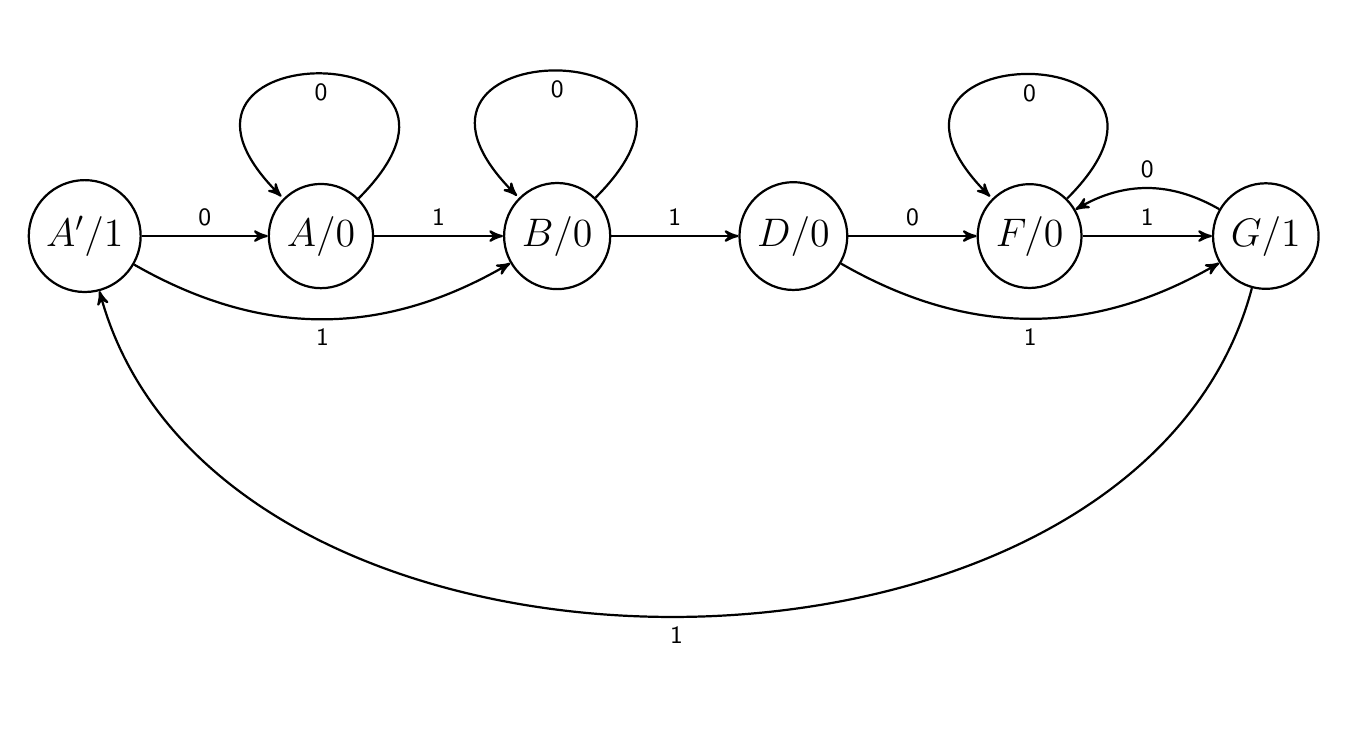
\begin{tikzpicture}[->,>=stealth',auto,node distance=3cm,
  thick,main node/.style={circle,draw,font=\sffamily\Large\bfseries}]
	    \node[main node] (1) {$A/0$};
  		\node[main node] (2) [right of=1] {$B/0$};
  		\node[main node] (3) [right of=2] {$D/0$};
  		\node[main node] (4) [right of=3] {$F/0$};
  		\node[main node] (5) [right of=4] {$G/1$};
  		\node[main node] (6) [ left of=1] {$A'/1$};

  		\path[every node/.style={font=\sffamily\small}]
    	(1) edge node [right, above] {1} (2)
    	(1) edge[loop] node[right, below] {0} (1)
    	(2) edge node [right, above] {1} (3)
    	(2) edge[loop] node[right, below] {0} (2)
    	(3) edge node [right, above] {0} (4)
    	(3) edge[bend right] node [below] {1} (5)
    	(4) edge node [right, above] {1} (5)
    	(4) edge[loop] node[right, below] {0} (4)    	
    	(5) edge[bend right] node [left, above] {0} (4)
    	(5) edge[bend left = 75] node [below] {1} (6)
    	(6) edge [bend right] node [right, below] {1} (2)
    	(6) edge node [right, above] {0} (1);
	\end{tikzpicture}
	\subsection{}
	%\begin{multicols}{2}[\textbf{Zustandsdiagramme}]

	Mealy\\
	\begin{tabular}{c c c c}
	\hline
	$S$ & $x$ & $S'$ & $y$\\	
	\hline
	$A$ & $0$ & $A$ & $0$\\
	$A$ & $1$ & $B$ & $0$\\
	$B$ & $0$ & $C$ & $0$\\
	$B$ & $1$ & $D$ & $0$\\
	$C$ & $0$ & $B$ & $0$\\
	$C$ & $1$ & $D$ & $0$\\
	$D$ & $0$ & $F$ & $0$\\
	$D$ & $1$ & $G$ & $1$\\
	$F$ & $0$ & $E$ & $0$\\
	$F$ & $1$ & $G$ & $0$\\
	$E$ & $0$ & $F$ & $0$\\
	$E$ & $1$ & $G$ & $0$\\
	$G$ & $0$ & $G$ & $0$\\
	$G$ & $1$ & $A$ & $1$\\
	\hline
	\end{tabular}
	\phantom{xxxxxxxxxxxxxxxxxxxxxxxxxxxxxxxxxxxxxxx}
	\begin{tabular}{c c c c}
	Moore\\
	\hline
	$S$ & $x$ & $S'$ & $y$ \\	
	\hline
	$A$ & $0$ & $A $& $0$\\
	$A$ & $1$ & $B $& $0$\\
	$B$ & $0$ & $B $& $0$\\
	$B$ & $1$ & $D $& $0$\\
	$D$ & $0$ & $F $& $0$\\
	$D$ & $1$ & $G $& $0$\\
	$F$ & $0$ & $F $& $0$\\
	$F$ & $1$ & $G $& $0$\\
	$G$ & $0$ & $F $& $1$\\
	$G$ & $1$ & $A'$& $1$\\
	$A'$& $0$ & $A$ & $0$\\
	$A'$& $1$ & $B$ & $0$\\
	\hline
	\end{tabular}
	\\~\\	


	\subsection{}
	Umkodieren von $\mathbb{S}$ in binäre Zustände $Q \subseteq\{0, 1\}^k$ mit $k = \log_2\left(\vert\mathbb{S}\vert\right)$\\~\\

	\begin{tabular}{c c c c}
	Mealy\\
	\hline
	$S$ & $x$ & $S'$ & $y$ \\	
	\hline
	\textcolor{red}{$A$} & $0$ & $A$ & $0$\\
	\textcolor{red}{$A$} & $1$ & $B$ & $0$\\
	\textcolor{red}{$B$} & $0$ & $B$ & $0$\\
	\textcolor{red}{$B$} & $1$ & $D$ & $0$\\
	\textcolor{red}{$D$} & $0$ & $F$ & $0$\\
	\textcolor{red}{$D$} & $1$ & $G$ & $1$\\
	\textcolor{red}{$F$} & $0$ & $F$ & $0$\\
	\textcolor{red}{$F$} & $1$ & $G$ & $0$\\
	\textcolor{red}{$G$} & $0$ & $G$ & $0$\\
	\textcolor{red}{$G$} & $1$ & $A$ & $1$\\
	\hline
	\end{tabular}
	\phantom{---------------------}$\longrightarrow$\phantom{-------------------}
	\begin{tabular}{*{8}{c}}
	Mealy\\
	\hline
	$\ind{q_2}$ & $\ind{q_1}$ & $\ind{q_0}$ & $x$ & $\ind{q'_2}$ & $\ind{q'_1}$ &$\ind{q'_0}$ & $y$ \\	
	\hline
	\textcolor{red}{$0$} & \textcolor{red}{$0$} & \textcolor{red}{$0$} & $0$ & $0$ & $0$ & $0$ & $0$\\
	\textcolor{red}{$0$} & \textcolor{red}{$0$} & \textcolor{red}{$0$} & $1$ & $0$ & $0$ & $1$ & $0$\\
	\textcolor{red}{$0$} & \textcolor{red}{$0$} & \textcolor{red}{$1$} & $0$ & $0$ & $0$ & $1$ & $0$\\
	\textcolor{red}{$0$} & \textcolor{red}{$0$} & \textcolor{red}{$1$} & $1$ & $0$ & $1$ & $0$ & $0$\\
	\textcolor{red}{$0$} & \textcolor{red}{$1$} & \textcolor{red}{$0$} & $0$ & $0$ & $1$ & $1$ & $0$\\
	\textcolor{red}{$0$} & \textcolor{red}{$1$} & \textcolor{red}{$0$} & $1$ & $1$ & $0$ & $0$ & $1$\\
	\textcolor{red}{$0$} & \textcolor{red}{$1$} & \textcolor{red}{$1$} & $0$ & $0$ & $1$ & $1$ & $0$\\
	\textcolor{red}{$0$} & \textcolor{red}{$1$} & \textcolor{red}{$1$} & $1$ & $1$ & $0$ & $0$ & $0$\\
	\textcolor{red}{$1$} & \textcolor{red}{$0$} & \textcolor{red}{$0$} & $0$ & $0$ & $0$ & $1$ & $0$\\
	\textcolor{red}{$1$} & \textcolor{red}{$0$} & \textcolor{red}{$0$} & $1$ & $0$ & $0$ & $0$ & $1$\\
	\hline
	\end{tabular}

	\subsection{}
	J-K-FlipFlop, da Zusand J = K = 1 erlaubt und ferner don't cares entstehen. D Flipfop hat des Weiteren nur einen einzigen Eingang, daher uninteressant. 
	Es werden 3 J-K-Flipflops benötigt.

	\subsection{}
	\begin{tabular}{*{12}{r}}
	Mealy\\
	\hline
	$\ind{q_2}$ & $\ind{q_1}$ & $\ind{q_0}$ & $x$ & $\ind{q'_2}$ & $\ind{q'_1}$ &$\ind{q'_0}$ & $\ind{J_2}$$\ind{K_2}$ & $\ind{J_1}$$\ind{K_1}$ & $\ind{J_0}$$\ind{K_0}$\\	
	\hline
	$0$& $0$ & $0$ & $0$ & $0$ & $0$ & $0$ & \textcolor{red}{$0$} \textcolor{red}{$d$} & \textcolor{red}{$0$} \textcolor{red}{$d$} & \textcolor{red}{$0$} \textbf{{\color{red}{$d$}}}\\%1
	$0$& $0$ & $0$ & $1$ & $0$ & $0$ & $1$ & \textcolor{red}{$0$} \textcolor{red}{$d$} & \textcolor{red}{$0$} \textcolor{red}{$d$} & \textcolor{red}{$1$} \textcolor{red}{$d$}\\%2
	$0$& $0$ & $1$ & $0$ & $0$ & $0$ & $1$ & \textcolor{red}{$0$} \textcolor{red}{$d$} & \textcolor{red}{$0$} \textcolor{red}{$d$} & \textcolor{red}{$d$} \textcolor{red}{$0$}\\%3
	$0$& $0$ & $1$ & $1$ & $0$ & $1$ & $0$ & \textcolor{red}{$0$} \textcolor{red}{$d$} & \textcolor{red}{$1$} \textcolor{red}{$d$} & \textcolor{red}{$d$} \textcolor{red}{$1$}\\%4
	$0$& $1$ & $0$ & $0$ & $0$ & $1$ & $1$ & \textcolor{red}{$0$} \textcolor{red}{$d$} & \textcolor{red}{$d$} \textcolor{red}{$0$} & \textcolor{red}{$1$} \textcolor{red}{$0$}\\%5
	$0$& $1$ & $0$ & $1$ & $1$ & $0$ & $0$ & \textcolor{red}{$1$} \textcolor{red}{$0$} & \textcolor{red}{$d$} \textcolor{red}{$1$} & \textcolor{red}{$d$} \textcolor{red}{$1$}\\%6
	$0$& $1$ & $1$ & $0$ & $0$ & $1$ & $1$ & \textcolor{red}{$d$} \textcolor{red}{$1$} & \textcolor{red}{$1$} \textcolor{red}{$d$} & \textcolor{red}{$1$} \textcolor{red}{$d$}\\%7
	$0$& $1$ & $1$ & $1$ & $1$ & $0$ & $0$ & \textcolor{red}{$1$} \textcolor{red}{$d$} & \textcolor{red}{$d$} \textcolor{red}{$1$} & \textcolor{red}{$d$} \textcolor{red}{$1$}\\%8
	$1$& $0$ & $0$ & $0$ & $0$ & $0$ & $1$ & \textcolor{red}{$d$} \textcolor{red}{$1$} & \textcolor{red}{$0$} \textcolor{red}{$d$} & \textcolor{red}{$1$} \textcolor{red}{$d$}\\
	$1$& $0$ & $0$ & $1$ & $0$ & $0$ & $0$ & \textcolor{red}{$0$} \textcolor{red}{$d$} & \textcolor{red}{$0$} \textcolor{red}{$d$} & \textcolor{red}{$d$} \textcolor{red}{$1$}\\
	\hline									
	\end{tabular}

	\subsection{}
	\phantom{xxxx\\}

	 Ausgabegleichung:\\  

	 $y = \left(\overline{\ind{q_2}} \cdot \ind{q_1} \cdot \overline{\ind{q_0}} \cdot x\right) + \left(\ind{q_2} \cdot \overline{\ind{q_1}} \cdot \overline{\ind{q_0}} \cdot x\right)$\\

	 Ansteuerungsgleichungen:\\ 

	 $\ind{J_0} = (\ind{q_1} \cdot \overline{\ind{q_2}} \cdot \overline{x}) + (\overline{\ind{q_0}} \cdot \overline{\ind{q_1}} \cdot {q_2}) + (\overline{\ind{q_0}} \cdot \overline{\ind{q_1}} \cdot x)$\\

	 $\ind{K_0} = (\ind{q_0} \cdot \overline{\ind{q_2}} \cdot x) + (\overline{\ind{q_0}} \cdot \overline{\ind{q_1}} \cdot x) + ({q_1} \cdot \overline{\ind{q_2}} \cdot x)$\\
	 
	 $\ind{J_1} = (\ind{q_0} \cdot \overline{\ind{q_2}} \cdot x)$\\
	 
	 $\ind{K_1} = (\ind{q_1} \cdot \overline{\ind{q_2}} \cdot x)$ \\

	 $\ind{J_2} = (\ind{q_1} \cdot \overline{\ind{q_2}} \cdot x)$\\
	 
	 $\ind{K_2} = (\ind{q_0} \cdot \ind{q_1} \cdot \overline{\ind{q_2}}) + (\overline{\ind{q_0}} \cdot \overline{\ind{q_1}} \cdot \overline{\ind{q_2}})$\\~\\





	%\end{multicols}
\end{document}